% main.tex -- the descriptive sweep over the shape of the size distribution.
% EVERY result number is a macro from numbers.tex, which paper/extract_numbers.py
% prints from the committed artifacts (out/sweep_descriptive.txt, out/grade_fabric.txt,
% out/mixture.txt, out/phase2_fits.csv). test_paper_numbers.py fails the build if a
% typed digit appears outside the design-token allowlist. Figures come from
% paper/make_paper_figures.py and regenerate byte-identically.
\documentclass[reprint,aps,pre,amsmath,amssymb,superscriptaddress,longbibliography,nofootinbib,floatfix]{revtex4-2}

\usepackage{graphicx}
\usepackage{bm}
\usepackage[colorlinks=true,linkcolor=blue,citecolor=blue,urlcolor=blue]{hyperref}
\graphicspath{{figures/}}
% generated by paper/extract_numbers.py -- do not edit; every value is printed from an artifact
\newcommand{\dPhiJLogn}{+0.0621}
\newcommand{\dPhiJLognSe}{0.0026}
\newcommand{\nSeedsLogn}{3}
\newcommand{\phiJLognZero}{0.5745}
\newcommand{\phiJLognZeroSe}{0.0004}
\newcommand{\phiJLognHalf}{0.6366}
\newcommand{\phiJLognHalfSe}{0.0023}
\newcommand{\dPhiJUnif}{+0.0242}
\newcommand{\dPhiJUnifSe}{0.0008}
\newcommand{\nSeedsUnif}{3}
\newcommand{\phiJUnifZero}{0.5751}
\newcommand{\phiJUnifZeroSe}{0.0008}
\newcommand{\phiJUnifHalf}{0.5993}
\newcommand{\phiJUnifHalfSe}{0.0008}
\newcommand{\dPhiJBidi}{+0.0139}
\newcommand{\dPhiJBidiSe}{0.0025}
\newcommand{\nSeedsBidi}{3}
\newcommand{\phiJBidiZero}{0.5751}
\newcommand{\phiJBidiZeroSe}{0.0008}
\newcommand{\phiJBidiHalf}{0.5890}
\newcommand{\phiJBidiHalfSe}{0.0020}
\newcommand{\ratioPhiJ}{4.47}
\newcommand{\ratioPhiJInvVar}{5.51}
\newcommand{\ratioPhiJPeak}{2.89}
\newcommand{\anovaFPhiJ}{144.7}
\newcommand{\anovaPPhiJ}{0.0000}
\newcommand{\welchTPhiJ}{13.5}
\newcommand{\welchTNomPhiJ}{2.78}
\newcommand{\welchTCalPhiJ}{5.87}
\newcommand{\zeroSkewDiffHalf}{+0.0103}
\newcommand{\zeroSkewSeHalf}{0.0017}
\newcommand{\zeroSkewTHalf}{6.02}
\newcommand{\zeroSkewNResolved}{3}
\newcommand{\zeroSkewNCv}{5}
\newcommand{\welchFprNomPhiJ}{21.4}
\newcommand{\tCritTwoDof}{4.303}
\newcommand{\pAbsTgtTwoDof}{0.184}
\newcommand{\anovaPZall}{0.14}
\newcommand{\anovaPZnr}{0.10}
\newcommand{\anovaPRat}{0.12}
\newcommand{\welchTFmean}{3.96}
\newcommand{\welchTCalFmean}{5.95}
\newcommand{\ratioZall}{1.10}
\newcommand{\ratioRat}{1.09}
\newcommand{\ratioZnr}{2.33}
\newcommand{\orderSurvivePct}{32}
\newcommand{\orderDraws}{20000}
\newcommand{\zallIdentityWorstRows}{0.0147}
\newcommand{\nShardFiles}{158}
\newcommand{\nRecords}{717}
\newcommand{\nDedup}{635}
\newcommand{\nConflicts}{14}
\newcommand{\nConflictRecords}{15}
\newcommand{\nSelectedRecords}{252}
\newcommand{\nSelected}{217}
\newcommand{\nRecappedCells}{35}
\newcommand{\nRecappedMaxMult}{2}
\newcommand{\nConflictsSelected}{5}
\newcommand{\conflictWorstDphi}{0.0040}
\newcommand{\conflictWorstDphiScale}{1.9}
\newcommand{\zallIdentityWorst}{0.0347}
\newcommand{\zallIdentityWorstN}{217}
\newcommand{\ratLognZero}{0.039}
\newcommand{\ratLognZeroSe}{0.003}
\newcommand{\ratLognZeroN}{3}
\newcommand{\znrLognZero}{5.111}
\newcommand{\znrLognZeroSe}{0.022}
\newcommand{\znrLognZeroN}{3}
\newcommand{\zallLognZero}{4.911}
\newcommand{\zallLognZeroSe}{0.034}
\newcommand{\zallLognZeroN}{3}
\newcommand{\ratLognThree}{0.221}
\newcommand{\ratLognThreeSe}{0.011}
\newcommand{\ratLognThreeN}{3}
\newcommand{\znrLognThree}{5.029}
\newcommand{\znrLognThreeSe}{0.007}
\newcommand{\znrLognThreeN}{3}
\newcommand{\zallLognThree}{3.918}
\newcommand{\zallLognThreeSe}{0.062}
\newcommand{\zallLognThreeN}{3}
\newcommand{\ratLognHalf}{0.448}
\newcommand{\ratLognHalfSe}{0.010}
\newcommand{\ratLognHalfN}{3}
\newcommand{\znrLognHalf}{4.922}
\newcommand{\znrLognHalfSe}{0.026}
\newcommand{\znrLognHalfN}{3}
\newcommand{\zallLognHalf}{2.734}
\newcommand{\zallLognHalfSe}{0.053}
\newcommand{\zallLognHalfN}{3}
\newcommand{\ratUnifZero}{0.040}
\newcommand{\ratUnifZeroSe}{0.003}
\newcommand{\ratUnifZeroN}{3}
\newcommand{\znrUnifZero}{5.118}
\newcommand{\znrUnifZeroSe}{0.026}
\newcommand{\znrUnifZeroN}{3}
\newcommand{\zallUnifZero}{4.912}
\newcommand{\zallUnifZeroSe}{0.035}
\newcommand{\zallUnifZeroN}{3}
\newcommand{\ratUnifThree}{0.234}
\newcommand{\ratUnifThreeSe}{0.008}
\newcommand{\ratUnifThreeN}{3}
\newcommand{\znrUnifThree}{5.037}
\newcommand{\znrUnifThreeSe}{0.012}
\newcommand{\znrUnifThreeN}{3}
\newcommand{\zallUnifThree}{3.866}
\newcommand{\zallUnifThreeSe}{0.032}
\newcommand{\zallUnifThreeN}{3}
\newcommand{\ratUnifHalf}{0.423}
\newcommand{\ratUnifHalfSe}{0.010}
\newcommand{\ratUnifHalfN}{3}
\newcommand{\znrUnifHalf}{5.037}
\newcommand{\znrUnifHalfSe}{0.018}
\newcommand{\znrUnifHalfN}{3}
\newcommand{\zallUnifHalf}{2.912}
\newcommand{\zallUnifHalfSe}{0.057}
\newcommand{\zallUnifHalfN}{3}
\newcommand{\ratBidiZero}{0.040}
\newcommand{\ratBidiZeroSe}{0.003}
\newcommand{\ratBidiZeroN}{3}
\newcommand{\znrBidiZero}{5.118}
\newcommand{\znrBidiZeroSe}{0.026}
\newcommand{\znrBidiZeroN}{3}
\newcommand{\zallBidiZero}{4.912}
\newcommand{\zallBidiZeroSe}{0.035}
\newcommand{\zallBidiZeroN}{3}
\newcommand{\ratBidiThree}{0.270}
\newcommand{\ratBidiThreeSe}{0.001}
\newcommand{\ratBidiThreeN}{3}
\newcommand{\znrBidiThree}{5.002}
\newcommand{\znrBidiThreeSe}{0.020}
\newcommand{\znrBidiThreeN}{3}
\newcommand{\zallBidiThree}{3.654}
\newcommand{\zallBidiThreeSe}{0.020}
\newcommand{\zallBidiThreeN}{3}
\newcommand{\ratBidiHalf}{0.458}
\newcommand{\ratBidiHalfSe}{0.001}
\newcommand{\ratBidiHalfN}{3}
\newcommand{\znrBidiHalf}{5.001}
\newcommand{\znrBidiHalfSe}{0.030}
\newcommand{\znrBidiHalfN}{3}
\newcommand{\zallBidiHalf}{2.718}
\newcommand{\zallBidiHalfSe}{0.014}
\newcommand{\zallBidiHalfN}{3}
\newcommand{\pairPhiA}{0.6042}
\newcommand{\pairPhiASe}{0.0032}
\newcommand{\pairPhiB}{0.6677}
\newcommand{\pairPhiBSe}{0.0006}
\newcommand{\pairDPhi}{+0.0635}
\newcommand{\pairDPhiSe}{0.0032}
\newcommand{\pairScale}{30.2}
\newcommand{\phiScale}{2.1\times10^{-3}}
\newcommand{\pairFillingPred}{+0.0604}
\newcommand{\pairCvAgree}{5.6\times10^{-17}}
\newcommand{\nMixCells}{123}
\newcommand{\pairCv}{0.500}
\newcommand{\pairXsA}{0.0357}
\newcommand{\pairXsB}{0.25}
\newcommand{\pairNsmallA}{0.500}
\newcommand{\pairNsmallB}{0.900}
\newcommand{\pairSkewA}{0.00}
\newcommand{\pairSkewB}{+2.67}
\newcommand{\mixMinPhaseCount}{50}
\newcommand{\mixNProd}{1500}
\newcommand{\mixDroppedRatio}{3}
\newcommand{\mixDroppedXs}{0.6}
\newcommand{\mixDroppedNminor}{36.1}
\newcommand{\mixEndpoint}{0.5940}
\newcommand{\mixPeakRThree}{0.6763}
\newcommand{\mixPeakXsRThree}{0.30}
\newcommand{\mixPeakExcRThree}{+0.0823}
\newcommand{\mixPeakRTwo}{0.6317}
\newcommand{\mixPeakXsRTwo}{0.40}
\newcommand{\mixPeakExcRTwo}{+0.0377}
\newcommand{\pairDPhiMuZero}{+0.0643}
\newcommand{\pairDPhiMuZeroSe}{0.0011}
\newcommand{\pairScaleMuZero}{30.6}
\newcommand{\pairPhiAMuZero}{0.6587}
\newcommand{\pairPhiBMuZero}{0.7230}
\newcommand{\betaMuThree}{0.5947}
\newcommand{\betaMuZero}{0.6413}
\newcommand{\fabSlopeLogn}{+0.197}
\newcommand{\fabSlopeLognSe}{0.225}
\newcommand{\fabResolveLogn}{0.23}
\newcommand{\fabMeanTLogn}{0.44}
\newcommand{\fabNLogn}{72}
\newcommand{\fabSlopeUnif}{-0.046}
\newcommand{\fabSlopeUnifSe}{0.191}
\newcommand{\fabResolveUnif}{0.19}
\newcommand{\fabMeanTUnif}{0.42}
\newcommand{\fabNUnif}{72}
\newcommand{\fabSlopeBidi}{+0.117}
\newcommand{\fabSlopeBidiSe}{0.194}
\newcommand{\fabResolveBidi}{0.19}
\newcommand{\fabMeanTBidi}{0.46}
\newcommand{\fabNBidi}{72}
\newcommand{\fabRegisteredResolve}{0.5}
\newcommand{\fabCells}{216}
\newcommand{\fabSeeds}{12}
\newcommand{\anisoSlopeLogn}{+0.0108}
\newcommand{\floorSlopeLogn}{+0.0106}
\newcommand{\anisoMinusFloorLogn}{+0.0002}
\newcommand{\anisoMinusFloorLognSe}{0.0029}
\newcommand{\fabSlopeLognDropFlagged}{-0.070}
\newcommand{\fabSlopeLognDropFlaggedSe}{0.265}
\newcommand{\dMaxOverLFlag}{0.25}
\newcommand{\fabFlaggedLogn}{34}
\newcommand{\fabFlaggedLognOf}{106}
\newcommand{\fabFlaggedTopLogn}{12}
\newcommand{\fabFlaggedTopLognOf}{12}
\newcommand{\fabFlaggedLognPrimary}{23}
\newcommand{\fabFlaggedLognPrimaryOf}{72}
\newcommand{\fabFlaggedTopLognPooled}{16}
\newcommand{\fabFlaggedTopLognPooledOf}{16}
\newcommand{\fabFlaggedUnif}{0}
\newcommand{\fabFlaggedUnifOf}{103}
\newcommand{\fabFlaggedTopUnif}{0}
\newcommand{\fabFlaggedTopUnifOf}{12}
\newcommand{\fabFlaggedUnifPrimary}{0}
\newcommand{\fabFlaggedUnifPrimaryOf}{72}
\newcommand{\fabFlaggedTopUnifPooled}{0}
\newcommand{\fabFlaggedTopUnifPooledOf}{13}
\newcommand{\fabFlaggedBidi}{0}
\newcommand{\fabFlaggedBidiOf}{108}
\newcommand{\fabFlaggedTopBidi}{0}
\newcommand{\fabFlaggedTopBidiOf}{12}
\newcommand{\fabFlaggedBidiPrimary}{0}
\newcommand{\fabFlaggedBidiPrimaryOf}{72}
\newcommand{\fabFlaggedTopBidiPooled}{0}
\newcommand{\fabFlaggedTopBidiPooledOf}{18}
\newcommand{\fabKwPLogn}{0.73}
\newcommand{\fabLevenePLogn}{0.048}
\newcommand{\fabKwPUnif}{1.00}
\newcommand{\fabLevenePUnif}{0.405}
\newcommand{\fabKwPBidi}{0.78}
\newcommand{\fabLevenePBidi}{0.678}
\newcommand{\ratRiseLogn}{11.4}
\newcommand{\znrDropLogn}{0.189}
\newcommand{\ratRiseUnif}{10.5}
\newcommand{\znrDropUnif}{0.081}
\newcommand{\ratRiseBidi}{11.3}
\newcommand{\znrDropBidi}{0.117}
\newcommand{\nGrains}{1500}
\newcommand{\muP}{0.3}
\newcommand{\poisson}{0.30}
\newcommand{\unbalancedTol}{0.02}
\newcommand{\relStressTol}{2\times10^{-3}}
\newcommand{\dtSafety}{0.5}
\newcommand{\maxIter}{200000}
\newcommand{\newtonDamping}{0.4}
\newcommand{\rattlerK}{2}
\newcommand{\truncLo}{0.2}
\newcommand{\truncHi}{5.0}
\newcommand{\pHatFitMax}{1.1\times10^{-3}}
\newcommand{\nRungs}{4}
\newcommand{\pHatTop}{1\times10^{-3}}
\newcommand{\pHatBottom}{3\times10^{-5}}
\newcommand{\rMin}{0.85}
\newcommand{\uniformCvMax}{0.577}
\newcommand{\bidiRatioHalf}{3}
\newcommand{\bidiFinesVolHalf}{0.036}
\newcommand{\phiJFrictionless}{0.6324}
\newcommand{\phiJFrictionlessSe}{0.0004}
\newcommand{\nFrictionless}{3}
\newcommand{\phiJMonoMuThree}{0.5745}
\newcommand{\phiJMonoMuThreeSe}{0.0004}
\newcommand{\nMonoMuThree}{3}
\newcommand{\phiJMonoTieBreak}{0.0015}
\newcommand{\nMonoTieBreakSeeds}{2}
\newcommand{\rcpLiterature}{0.64}
\newcommand{\fillPa}{1.02}
\newcommand{\fillPb}{1.50}


% one symbol, one meaning
\newcommand{\phiJ}{\phi_{J}}
\newcommand{\pHat}{\hat{p}}
\newcommand{\Znr}{Z_{\mathrm{nr}}}
\newcommand{\Zall}{Z_{\mathrm{all}}}
\newcommand{\fr}{f_{r}}
\newcommand{\Tnr}{T_{\mathrm{nr}}}
\newcommand{\mup}{\mu_{p}}
\newcommand{\CV}{\mathrm{CV}}
\newcommand{\Xs}{X_{s}}
\newcommand{\dten}{d_{10}}

\begin{document}

\title{The jamming fraction of frictional spheres depends on the shape of the size distribution, not only on its width: a descriptive sweep}

\author{A.~Author} % TODO: author name and affiliation are the author's to fill in
\affiliation{Affiliation}

\date{\today}

\begin{abstract}
We compress periodic packings of $N=\nGrains$ frictional spheres ($\mup=\muP$) to jamming under isotropic stress control for three families of particle-size distribution held at the same number-mean diameter and the same number coefficient of variation $\CV$: lognormal, uniform, and a number-symmetric bidisperse mixture.
With the packing fraction extrapolated to zero pressure, the jamming fraction $\phiJ$ rises with $\CV$ in every family, but by amounts that differ across families by a factor of three to five over $\CV=0\to0.5$, depending on how the endpoint is defined ($\dPhiJLogn\pm\dPhiJLognSe$ lognormal, $\dPhiJUnif\pm\dPhiJUnifSe$ uniform, $\dPhiJBidi\pm\dPhiJBidiSe$ bidisperse; seed-paired means $\pm$ s.e.).
The shape of the distribution therefore moves $\phiJ$ more than a fourfold change of its width does within any one family, so the width alone is not the control parameter.
Above jamming, at fixed pressure, the picture is the opposite.
Polydispersity removes grains from the load-bearing network, with the rattler fraction rising about elevenfold in every family, while the coordination number and contact-orientation statistic of the surviving backbone are family-independent within uncertainty; a pre-registered test for a change in backbone orientational order returns the null at its registered resolving power.
A composition sweep over binary mixtures shows why the width fails.
Two mixtures with the same two diameters, the same size ratio and identical number $\CV$, differing in which species carries the volume, jam $\pairDPhi\pm\pairDPhiSe$ apart, $\pairScale$ times the protocol's run-to-run scatter; a Furnas-type interstitial-filling model with interaction exponents fixed in advance predicts $\pairFillingPred$ for that pair without a fitted parameter.
The jamming shift tracks how volume is distributed across size pairs, which no width descriptor of the number distribution records.
\end{abstract}

\maketitle

\section{Introduction}

The packing fraction at which a dense suspension of frictional particles jams, $\phiJ$, is the quantity a stress-dependent constitutive model needs before it can predict a viscosity: in the Wyart--Cates picture the viscosity diverges at a jamming fraction that interpolates, with stress, between a frictionless and a frictional value \cite{wyart2014discontinuous}.
For monodisperse spheres both limits are well characterised \cite{ohern2003jamming,silbert2010jamming,vanhecke2010jamming}.
Real suspensions are polydisperse.
The usual practice is to summarise the size distribution by one number, its width as a coefficient of variation, and to treat $\phiJ$ as a function of that.

For the frictionless random-close-packing problem, one number has been known to be insufficient for some time.
Desmond and Weeks showed that the skewness of the size distribution moves the close-packed fraction independently of its width \cite{desmond2014influence}; Farr and Groot built a predictive model that takes the whole distribution as input \cite{farr2009close}; Hopkins, Stillinger and Torquato showed that binary sphere packings attain an anomalously wide range of densities as ratio and composition vary \cite{hopkins2013disordered}; and the interstitial-filling account of maximum-density gradings goes back to Furnas \cite{furnas1931grading}.
What is missing for the frictional case relevant to suspension rheology is a controlled comparison in which the width is held fixed and only the shape is changed, together with a look at what the change in $\phiJ$ does to the contact network.

This paper reports that comparison.
It is a descriptive sweep, not a test of a theory: the design holds the number mean and number $\CV$ of the size distribution fixed across three families that differ in skewness and support, compresses each to jamming under one protocol, and reports $\phiJ$, the rattler fraction, the backbone coordination number and the backbone contact-orientation statistic as functions of $\CV$ for each family.
It then adds a composition sweep over binary mixtures, which is where the interpretation comes from.
Every number in the text is printed by the analysis scripts from the committed simulation output, and every statistical threshold is stated with the test that sets it.
Each figure regenerates byte-identically from one command.

\section{Methods}

\subsection{Packing protocol}

Packings are built with the open-source discrete-element code Yade \cite{smilauer2021yade} using the linear-spring Cundall--Strack contact law \cite{cundall1979discrete}.
Diameters are drawn from the chosen distribution with number-mean diameter $\dten=1$; material density and Young's modulus are unity; Poisson's ratio is $\poisson$; the interparticle friction coefficient is $\mup=\muP$.
$N=\nGrains$ spheres are placed in a periodic cell and compressed isotropically under stress control (Yade's \texttt{PeriTriaxController}) to a target reduced pressure $\pHat=p/E$, with velocity damping $\newtonDamping$, time step $\dtSafety$ of the critical step, and the run accepted when the unbalanced-force ratio is below $\unbalancedTol$ and the stress is within $\relStressTol$ of its target, or rejected if the iteration cap of $\maxIter$ is reached first.
The size distribution is truncated at $\truncLo\,\dten$ and $\truncHi\,\dten$.
A cell whose largest grain exceeds $\dMaxOverLFlag$ of the periodic box length is flagged as a finite-size risk; the flag is carried through every analysis and reported where it fires (Sec.~\ref{sec:fabric}).
The campaign's $\nShardFiles$ output shards hold $\nRecords$ records, $\nDedup$ after dropping failed runs and collapsing repeated cell keys; $\nConflicts$ keys ($\nConflictRecords$ records) were run more than once and returned different packing fractions from the same seed, all of them monodisperse cells, where the packing is most degenerate.
The rule is to keep the record with the higher iteration cap and otherwise the first in file order; $\nConflictsSelected$ of the affected keys enter the analysed set, and the largest disagreement among them is $\conflictWorstDphi$ in $\phi$, $\conflictWorstDphiScale$ times the run-to-run scatter, in a single seed at $\CV=0$.
That cell key carries the iteration cap, so a cell re-run at the raised cap survives the collapse twice: the $\nSelectedRecords$ records at $N=\nGrains$, $\mup=\muP$ that converged are $\nSelected$ distinct cells, $\nRecappedCells$ of them re-run under both caps.
The per-rung means, standard errors and seed counts reported below are taken over the $\nSelected$ cells, with the higher cap kept, so that a change of cap is never counted as an extra seed.

\subsection{Size-distribution families}

Three families are compared at matched number mean and matched number coefficient of variation $\CV$, at $\CV = 0, 0.1, \ldots, 0.5$:
\begin{itemize}
\item \emph{lognormal}, with positive skewness that grows with $\CV$;
\item \emph{uniform}, a symmetric (zero-skewness) distribution of half-width $\sqrt{3}\,\CV\,\dten$, which exists only for $\CV<\uniformCvMax$;
\item \emph{bidisperse}, two diameters $\dten(1\pm\CV)$ in equal number, also of zero skewness but with all its weight at the two extremes.
\end{itemize}
The last family deserves a warning that the results depend on.
Because it is symmetric by \emph{number}, its size ratio $(1+\CV)/(1-\CV)$ and its fines \emph{volume} fraction $(1-\CV)^3/[(1-\CV)^3+(1+\CV)^3]$ both move with $\CV$: at $\CV=0.5$ the size ratio is $\bidiRatioHalf$ and the small species carries only $\bidiFinesVolHalf$ of the volume.
The bidisperse family is therefore a one-parameter \emph{path} through the (size ratio, composition) plane of binary mixtures, and its $\CV=0.5$ member is a fines-poor mixture, not a representative bidisperse packing.
The composition sweep of Sec.~\ref{sec:binaries} exists to see the rest of that plane.

\subsection{Observables}

\paragraph{Jamming fraction.}
For each family, $\CV$ and seed a ladder of $\nRungs$ target pressures $\pHat = \pHatTop$ down to $\pHatBottom$ is compressed, and the packing fraction $\phi(\pHat)$ is fitted linearly in $\pHat$ over the rungs with $\pHat\le\pHatFitMax$ and extrapolated to $\pHat\to0$; the intercept is $\phiJ$ \cite{ohern2003jamming}.
A ladder is accepted only if its fit has $r^2\ge\rMin$ and a non-negative slope; the ladder-health gate (no negative slope, median $r^2$ above the bar) passes on all three families.
The linear form is a choice, and the paired differences reported below are differences of intercepts, so the conclusions do not rest on the exponent of the approach to jamming, which this data cannot determine.

\paragraph{Rattlers and the backbone.}
The remaining observables are read at the top rung $\pHat=\pHatTop$ rather than extrapolated, because they have no zero-pressure limit that the ladder resolves.
A grain with fewer than $k=\rattlerK$ load-bearing contacts is a rattler and is removed; removal is iterated to a fixed point \cite{ohern2003jamming,vanhecke2010jamming}.
The rattler fraction $\fr$, the mean coordination of the surviving backbone $\Znr$ and the mean coordination of all grains $\Zall$ are reported; $\Zall=(1-\fr)\Znr$ holds to within $\zallIdentityWorst$ on every cell, so $\Zall$ carries no information beyond the other two.

\paragraph{Contact orientation.}
For the backbone contacts the deviatoric fabric anisotropy $A$ is computed from the contact unit normals.
Because $E[A^2]=1/n$ exactly for $n$ independent unit normals, $A$ itself carries a finite-sample floor that rises as polydispersity removes contacts, in the same direction a restructuring signal would; the statistic reported is instead $\Tnr = n A^2$, which has $E[\Tnr]=1$ under the independent-normal null with no contact-count dependence.
Its \emph{absolute} value carries no claim, since contacts sharing a grain are not independent draws; only its dependence on $\CV$ is tested.
The fabric campaign has its own cells, $\fabSeeds$ seeds per family and $\CV$, $\fabCells$ cells in all, and its primary test was pre-registered as a null with a registered effect size of $\fabRegisteredResolve$ in $\Tnr$ over $\CV=0\to0.5$.

\subsection{Statistics}

Each family's $\CV=0\to0.5$ change is a \emph{paired} difference: the two ends share the seed, and the difference is taken per seed before averaging, so the shared draw cancels exactly.
With $\nSeedsLogn$ seeds per family the standard error carries two degrees of freedom and the two-sided critical value is $t=\tCritTwoDof$, not $2$; a flat $2\,\mathrm{s.e.}$ bar would be a test at level $\pAbsTgtTwoDof$.
An across-family ratio is quoted only if three gates pass: the smallest family change clears its own $t$ threshold (else the ratio's denominator is noise), a one-way ANOVA across families rejects a common change, and the specific max-versus-min pair carrying the ratio is separated by a Welch $t$ whose critical value is \emph{calibrated} for the fact that the pair was selected from the data---by simulating the channel under the null of a common value, applying the same argmax/argmin rule, and taking the upper $95\,\%$ point of the resulting Welch $t$.
The nominal Welch critical value is reported beside the calibrated one together with its true false-positive rate.

\section{Results}

\subsection{The jamming fraction follows the shape}
\label{sec:phij}

\begin{figure}
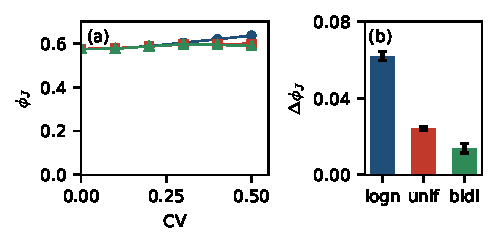
\includegraphics[width=\columnwidth]{fig1_phiJ.pdf}
\caption{\label{fig:phiJ}(a) Jamming fraction $\phiJ$ extrapolated to $\pHat\to0$ against the number $\CV$ of the size distribution for the lognormal (circles), uniform (squares) and number-symmetric bidisperse (triangles) families at matched number mean, $\mup=\muP$, $N=\nGrains$; mean $\pm$ s.e.\ over seeds. (b) The seed-paired change over $\CV=0\to0.5$ per family. Axes start at zero so that the family spread in (b) is read against the size of $\phiJ$ itself. The bidisperse point at $\CV=0.5$ is a size-ratio-$\bidiRatioHalf$ mixture with $\bidiFinesVolHalf$ of its volume in fines (see text).}
\end{figure}

Figure~\ref{fig:phiJ}(a) shows $\phiJ(\CV)$ for the three families.
All three start from monodisperse values that agree within seed scatter ($\phiJLognZero\pm\phiJLognZeroSe$ and $\phiJUnifZero\pm\phiJUnifZeroSe$; mean $\phiJMonoMuThree$ at $\mup=\muP$), and all rise with $\CV$; but the lognormal family rises to $\phiJLognHalf\pm\phiJLognHalfSe$ at $\CV=0.5$, the uniform family to $\phiJUnifHalf\pm\phiJUnifHalfSe$, and the bidisperse family reaches $\phiJBidiHalf\pm\phiJBidiHalfSe$ after passing through a maximum near $\CV=0.3$.
The paired $\CV=0\to0.5$ changes, Fig.~\ref{fig:phiJ}(b), are
\begin{align}
\Delta\phiJ^{\mathrm{logn}} &= \dPhiJLogn \pm \dPhiJLognSe, \nonumber\\
\Delta\phiJ^{\mathrm{unif}} &= \dPhiJUnif \pm \dPhiJUnifSe, \\
\Delta\phiJ^{\mathrm{bidi}} &= \dPhiJBidi \pm \dPhiJBidiSe, \nonumber
\end{align}
each over $\nSeedsLogn$ seeds.
The ratio of largest to smallest is $\ratioPhiJ$.
All three gates of the statistics section pass on this channel: the smallest change clears its $t$ threshold, the ANOVA gives $F=\anovaFPhiJ$ ($p=\anovaPPhiJ$ to four decimals), and the lognormal--bidisperse pair has Welch $t=\welchTPhiJ$ against a selection-calibrated critical value of $\welchTCalPhiJ$ (the nominal critical value, $\welchTNomPhiJ$, would have a false-positive rate of $\welchFprNomPhiJ\,\%$ under this selection rule).
$\phiJ$ is the only channel in the sweep that passes all three.

The number $\ratioPhiJ$ is a definition-dependent summary and two brackets belong beside it.
Weighting the seeds by the inverse variance of their own ladder fits instead of equally gives $\ratioPhiJInvVar$; the ANOVA becomes more significant under that weighting, not less.
Taking each family at its own peak over $\CV$ rather than at the $\CV=0.5$ endpoint---which matters for the non-monotone bidisperse family---gives $\ratioPhiJPeak$; that number is a maximum over noisy estimates and so is biased the other way.
The supportable statement is that the family spread is a factor of three to five, and that it exceeds the effect of $\CV$ within either zero-skewness family.

Two design-level checks anchor the protocol.
The monodisperse frictionless jamming fraction obtained by the same ladder extrapolation is $\phiJFrictionless\pm\phiJFrictionlessSe$ ($n=\nFrictionless$), to be compared with the random-close-packing value near $\rcpLiterature$ from the literature \cite{ohern2003jamming,silbert2010jamming}; the frictional value $\phiJMonoMuThree$ at $\mup=\muP$ sits below it, in the direction reported for frictional packs \cite{silbert2010jamming}.
The frictionless ladders are not monotone in $\pHat$ at this seed count, so this anchor is a check of the protocol's scale and not a result of the paper.
The uniform and bidisperse families share their $\CV=0$ cells, which is why their $\CV=0$ entries coincide in every table; their two paired changes therefore share a subtrahend, and a test that treats them as independent overstates the variance of their difference by twice the variance of the shared cell, i.e.\ errs on the conservative side.
The pair that carries the ratio, lognormal against bidisperse, shares no cell.

\subsection{Polydispersity removes grains; it does not restructure the backbone}
\label{sec:fabric}

\begin{figure*}
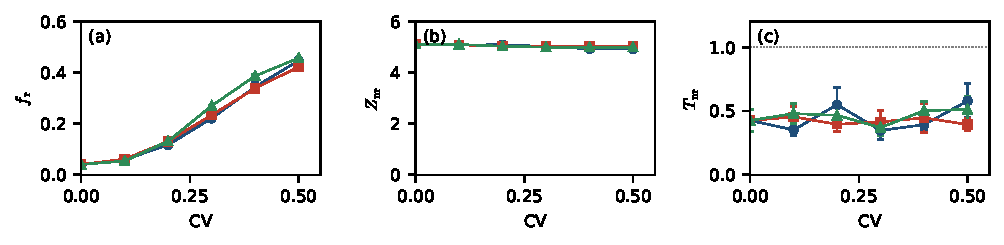
\includegraphics[width=\textwidth]{fig2_backbone.pdf}
\caption{\label{fig:backbone}Backbone observables at $\pHat=\pHatTop$, same symbols as Fig.~\ref{fig:phiJ}, mean $\pm$ s.e.\ over seeds. (a) Rattler fraction $\fr$ at $k=\rattlerK$. (b) Mean coordination of the surviving backbone $\Znr$. (c) The backbone contact-orientation statistic $\Tnr=nA^2$ from the fabric campaign ($\fabSeeds$ seeds); the dotted line is the independent-normal expectation $E[\Tnr]=1$. Panel (a) rises about elevenfold; (b) and (c) are flat within uncertainty.}
\end{figure*}

Figure~\ref{fig:backbone} shows what the same $\CV$ ladders do to the contact network.
The rattler fraction rises from $\ratLognZero\pm\ratLognZeroSe$ to $\ratLognHalf\pm\ratLognHalfSe$ in the lognormal family, a factor of $\ratRiseLogn$, and by factors of $\ratRiseUnif$ and $\ratRiseBidi$ in the uniform and bidisperse families: by $\CV=0.5$ close to half the grains carry no load in every family.
The backbone coordination hardly moves.
$\Znr$ falls by $\znrDropLogn$ (lognormal), $\znrDropUnif$ (uniform) and $\znrDropBidi$ (bidisperse) from $\CV=0$ values near $\znrLognZero$.
The all-grain coordination $\Zall$ falls by about two, but that is the identity $\Zall=(1-\fr)\Znr$ applied to the rise in $\fr$, not an independent observation.

Across families, none of these channels resolves a shape dependence: the ANOVA $p$-values for a family-dependent $\CV=0\to0.5$ change are $\anovaPZall$ ($\Zall$), $\anovaPZnr$ ($\Znr$) and $\anovaPRat$ ($\fr$).
The mean contact force does reject a common change ($F$ test), but its max--min pair fails the selection-calibrated Welch gate (Welch $t=\welchTFmean$ against a calibrated $\welchTCalFmean$), so it is not quoted either.
The strong shape dependence of $\phiJ$ is thus not visible in what happens to the load-bearing network at fixed pressure above jamming; three families whose $\CV=0\to0.5$ shifts in $\phiJ$ range from $\dPhiJBidi$ to $\dPhiJLogn$ lose grains from the backbone at the same rate and keep the same backbone coordination.

The fabric campaign tests the remaining possibility, that the surviving backbone reorganises its contact orientations.
The pre-registered primary statistic is the per-family OLS slope of $\Tnr$ against $\CV$, with the null predicted; the registered verdict grammar calls a slope a drift if it exceeds twice its standard error and calls the null informative only if the achieved resolving power over the $\CV$ range is at or below the registered effect size $\fabRegisteredResolve$.
The slopes are $\fabSlopeLogn\pm\fabSlopeLognSe$ (lognormal, $n=\fabNLogn$ cells), $\fabSlopeUnif\pm\fabSlopeUnifSe$ (uniform, $n=\fabNUnif$) and $\fabSlopeBidi\pm\fabSlopeBidiSe$ (bidisperse, $n=\fabNBidi$), with achieved resolving powers $\fabResolveLogn$, $\fabResolveUnif$ and $\fabResolveBidi$: the null holds on all three families and is informative on all three.
The resolving power is twice the standard error of the slope multiplied by the $\CV$ range, which is $0.5$ here, so it is numerically the standard error already quoted and not a second, independent measurement.
A distribution-free Kruskal--Wallis test across the six $\CV$ rungs, which has power against a non-monotone dependence that an OLS slope would miss, gives $p=\fabKwPLogn$, $\fabKwPUnif$ and $\fabKwPBidi$.

Two caveats travel with the lognormal result.
First, $\fabFlaggedLognPrimary$ of the $\fabFlaggedLognPrimaryOf$ lognormal fabric cells on the primary rung carry the finite-size flag $d_{\max}/L>\dMaxOverLFlag$ ($\fabFlaggedLogn$ of $\fabFlaggedLognOf$ pooled over both rungs), and at $\CV=0.5$ all $\fabFlaggedTopLognOf$ primary-rung cells do ($\fabFlaggedTopLognPooled$ of $\fabFlaggedTopLognPooledOf$ pooled), against none in the two zero-skewness families; the lognormal tail at $N=\nGrains$ puts single grains across a quarter of the box.
Dropping the wholly flagged rung changes the lognormal slope to $\fabSlopeLognDropFlagged\pm\fabSlopeLognDropFlaggedSe$: the verdict survives, but the point estimate changes sign, so the lognormal slope must not be quoted as a number.
Second, Levene's test finds unequal variances of $\Tnr$ across $\CV$ in the lognormal family ($p=\fabLevenePLogn$, against $\fabLevenePUnif$ and $\fabLevenePBidi$ in the other two), so the Kruskal--Wallis column is the one to read there.
Finally, the raw anisotropy $A$ does rise with $\CV$ in the lognormal family, by $\anisoSlopeLogn$ per unit $\CV$; the $1/\sqrt{n}$ floor computed from the measured contact counts rises by $\floorSlopeLogn$, and the difference, $\anisoMinusFloorLogn\pm\anisoMinusFloorLognSe$, is zero.
The apparent rise in anisotropy is entirely finite-sample bookkeeping.

\subsection{Two mixtures with identical width descriptors}
\label{sec:binaries}

\begin{figure}
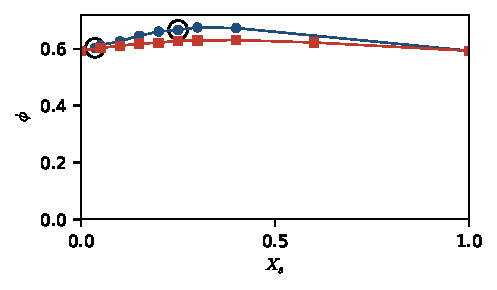
\includegraphics[width=\columnwidth]{fig3_binaries.pdf}
\caption{\label{fig:binaries}Packing fraction $\phi$ at $\pHat=\pHatTop$, $\mup=\muP$, $N=\nGrains$, for binary mixtures at size ratio $3$ (circles) and $2$ (squares) against the volume fraction of the small species $\Xs$; mean $\pm$ s.e.\ over seeds; both endpoints are the monodisperse pack. The two ringed points at ratio $3$ have the same two diameters and identical number $\CV$ and differ only in which species carries the volume.}
\end{figure}

The bidisperse family's non-monotone $\phiJ(\CV)$ is the signature of a quantity that depends on how volume is shared between size pairs rather than on any moment of the number distribution.
To see this directly, $\nMixCells$ cells were run at fixed size ratio across the full composition range (Fig.~\ref{fig:binaries}); $\phi$ is read at $\pHat=\pHatTop$, so these are packing fractions at a pressure, not extrapolated $\phiJ$, and the mono\-disperse endpoint is $\mixEndpoint$ rather than $\phiJMonoMuThree$.
A composition is admitted only if its minor species is expected to number at least $\mixMinPhaseCount$ grains at $N=\mixNProd$, a rule written into the campaign script before any cell was graded; one interior composition fails it, ratio $\mixDroppedRatio$ at $\Xs=\mixDroppedXs$ with $\mixDroppedNminor$ expected large grains, and is omitted from the figure.
At size ratio $3$ the packing fraction peaks at $\mixPeakRThree$ near $\Xs=\mixPeakXsRThree$, $\mixPeakExcRThree$ above the monodisperse value; at ratio $2$ it peaks at $\mixPeakRTwo$ near $\Xs=\mixPeakXsRTwo$, $\mixPeakExcRTwo$ above it.
This is the classical Furnas picture \cite{furnas1931grading,hopkins2013disordered}.

The decisive comparison is the ringed pair.
Mixture A is the bidisperse family's $\CV=0.5$ member: size ratio $3$, half the grains small by number ($n_s=\pairNsmallA$), fines volume fraction $\Xs=\pairXsA$.
Mixture B uses the same two diameters with $\Xs=\pairXsB$, which puts $n_s=\pairNsmallB$ of the grains in the small species.
Their number $\CV$s agree to $\pairCvAgree$, and their size ratio, span, and number of distinct diameters are identical by construction, so the width descriptors of the number distribution---$\CV$, $d_{\max}/d_{\min}$, the span---take the same value on both.
The skewness does not: a two-point distribution cannot hold both $\CV$ and skewness fixed at two compositions, and the number skewness is $\pairSkewA$ for A and $\pairSkewB$ for B.
The pair therefore separates composition from the width of the distribution, not from its asymmetry; the skewness axis is what the uniform and lognormal families of Sec.~\ref{sec:phij} compare at fixed $\CV$.
They jam at
\begin{equation}
\phi_A=\pairPhiA\pm\pairPhiASe,\qquad \phi_B=\pairPhiB\pm\pairPhiBSe,
\end{equation}
a difference $\Delta\phi=\pairDPhi\pm\pairDPhiSe$, which is $\pairScale$ times the protocol's own run-to-run scatter of $\phiScale$ measured on repeated monodisperse cells.
Any account of the jamming shift built from the width of the number distribution predicts exactly zero here; an account built on its skewness does not, and this pair cannot exclude one.
A linear packing model of the Furnas type, in which each size class packs at the measured monodisperse fraction and the interaction between classes is set by two size-ratio functions with exponents fixed in advance of the composition campaign at $\fillPa$ and $\fillPb$, the loosening- and wall-effect exponents of the compressible packing model as given in Ref.~\cite{diaz2021packing}, predicts $\pairFillingPred$ for this pair with no parameter fitted to it.
% [UNVERIFIED attribution] the two exponent values are printed in diaz2021packing (verified against the open full text, eqs. 26 and 33); whether they are de Larrard's own 1999 values or a later revision of the model has not been checked against the book (refs.bib annote).
% Re-checked 2026-09-17: still unresolved, and the reason is now in the annote -- there are two de Larrard 1999 publications (this CRC Press book and an LCPC monograph) and diaz2021packing cites the latter. The forms themselves: eq. 26 is b(x) = 1 - (1-x)^1.5 and eq. 33 is a(x) = sqrt(1 - (1-x)^1.02); the annote had the square root missing and is corrected. mixture_model.py always had it, so no number moves.
(Ref.~\cite{diaz2021packing} attributes these functions to de Larrard's compressible packing model, citing two earlier de Larrard sources, neither of which is Ref.~\cite{delarrard1999concrete}; we have checked neither de Larrard source, and what matters here is that the two values were held fixed before the pair was measured.)
The same pair at $\mup=0$ gives $\pairDPhiMuZero\pm\pairDPhiMuZeroSe$, $\pairScaleMuZero$ times the scatter, so the separation is not a frictional effect.

\section{Discussion}

The width of the size distribution is not the control parameter for $\phiJ$: at fixed width, three shapes give shifts spanning a factor of $\ratioPhiJ$ (between $\ratioPhiJPeak$ and $\ratioPhiJInvVar$ under the other two definitions of Sec.~\ref{sec:phij}), and the shift is not even monotone in width for one of them.
The contact network above jamming does not distinguish the shapes either: every family loses about the same fraction of its grains to the rattler population, keeps the same backbone coordination, and shows no change in backbone contact orientation at the registered resolving power.
What distinguishes them is how volume is apportioned across size pairs, which the binary sweep isolates: at identical width descriptors, moving a quarter of the volume into the fines changes $\phi$ by $\pairDPhi$, and a filling model with its exponents fixed in advance predicts the size of that change.
The pair does not hold the skewness fixed, so it separates composition from width, not from asymmetry.
Skewness is therefore not excluded as a control parameter by this sweep: the only test that could exclude it is the two zero-skewness families against each other ($\dPhiJUnif$ against $\dPhiJBidi$), and that pair has not been tested at the calibrated threshold.
What the pair does show is that the filling account, which uses the volume composition and not the skewness, predicts the separation.

This agrees with the frictionless literature: Desmond and Weeks found skewness to matter as much as width \cite{desmond2014influence}, and Farr and Groot's predictive model takes the entire distribution as input for the same reason \cite{farr2009close}.
It also removes an apparent conflict with a recent two-dimensional study whose abstract reports the shear-jamming point varying non-monotonically with polydispersity \cite{singh2025rigidity}: that study's distributions are normal, i.e.\ of zero skewness, and the zero-skewness families here also show the weakest and, for the bidisperse case, non-monotone response.
Shear jamming is a distinct route to rigidity from isotropic compression \cite{bi2011jamming}, so the comparison across dimensions, protocols and jamming points is qualitative.

The limits of the sweep are worth naming, and the bidisperse family is the first of them.
It is a path through the (ratio, composition) plane, and its $\CV=0.5$ member is a fines-poor mixture; the family's small $\Delta\phiJ$ is a property of that path, not of bidisperse packings in general, as Fig.~\ref{fig:binaries} makes plain.
The across-family spread is a range over three families, not a pairwise statement about any two: only the lognormal--bidisperse pair has been tested against the selection-calibrated threshold.
$\Znr$, $\fr$ and $\Tnr$ are read at a pressure, $\pHat=\pHatTop$, and the flat backbone coordination is a statement at that pressure; the zero-pressure isostatic limit is not resolved here.
The lognormal family at $\CV\ge0.3$ carries the finite-size flag at $N=\nGrains$, which touches the fabric slope (Sec.~\ref{sec:fabric}) and, through the same tail, may touch its $\phiJ$; a larger-$N$ repeat of that family is the obvious next cell to spend.
And the filling model's prediction is a single-pair comparison at exponents fixed in advance from one tabulated source; whether one set of interaction functions transfers across friction, size ratio and continuous distributions is a separate question that the present data can pose but not settle.

\section{Conclusions}

For frictional spheres compressed to jamming under one protocol, the jamming fraction responds to the shape of the size distribution at fixed width by a factor of three to five more than to a fourfold change of width within a zero-skewness family, and the response is not monotone in width for a number-symmetric bidisperse mixture.
Above jamming, polydispersity depopulates the load-bearing network without restructuring what remains: the rattler fraction rises about elevenfold in every family while the backbone coordination and contact orientation are family-independent and $\CV$-independent within the resolving power of the tests.
Two binary mixtures with identical width descriptors jam $\pairDPhi$ apart, $\pairScale$ times the protocol scatter, and a parameter-free filling model predicts the separation; the pair leaves the skewness free, so it rules out the width, not every moment.
A rheological model that summarises polydispersity by a coefficient of variation is therefore using a variable that does not determine $\phiJ$.
The volume distribution across size pairs, which the filling model reads, accounts for the one separation it was tested on.
Whether a lower-order descriptor such as the skewness could do the same is left open by the untested zero-skewness pair.

\begin{acknowledgments}
The simulation output, the analysis scripts that print every number in this paper, the figure scripts and their data tables, and the pre-registration documents for the fabric and composition campaigns are archived with the manuscript.
\end{acknowledgments}

\bibliography{refs}

\end{document}
